\documentclass[12pt,a4paper]{article}
\usepackage[utf8]{inputenc}
\usepackage[greek,english]{babel}
\usepackage{alphabeta} 
\usepackage[pdftex]{graphicx}
\usepackage[top=1in, bottom=1in, left=0.5in, right=0.5in]{geometry}
\linespread{1}
\setlength{\parskip}{8pt plus2pt minus2pt}
\widowpenalty 10000
\clubpenalty 10000
\newcommand{\eat}[1]{}
\newcommand{\HRule}{\rule{\linewidth}{0.5mm}}
\usepackage[official]{eurosym}
\usepackage{enumitem}
\setlist{nolistsep,noitemsep}
\usepackage[hidelinks]{hyperref}
\usepackage{cite}
\usepackage{lipsum}
\graphicspath{ {./images/} }
\usepackage{listings}
\usepackage{color}
\setlength{\parindent}{0pt}


\definecolor{dkgreen}{rgb}{0,0.6,0}
\definecolor{gray}{rgb}{0.5,0.5,0.5}
\definecolor{mauve}{rgb}{0.58,0,0.82}


\lstset{frame=tb,
	language=C,
	aboveskip=3mm,
	belowskip=3mm,
	showstringspaces=false,
	columns=flexible,
	basicstyle={\small\ttfamily},
	numbers=none,
	numberstyle=\tiny\color{gray},
	keywordstyle=\color{blue},
	commentstyle=\color{dkgreen},
	stringstyle=\color{mauve},
	breaklines=true,
	breakatwhitespace=true,
	tabsize=3
}



\begin{document}
	%===========================================================
\begin{titlepage}
	\begin{center}

		
		% Title
		\HRule \\[0.4cm]
		{ \LARGE 
			\textbf{ECE 351 Final Lab}\\[0.4cm]
		}
		\HRule \\[1.5cm]
		
		
		
		% Author
		{ \large
			Zachary Deluca \\[0.1cm]
			April 25th, 2023\\[0.1cm]
			%#\texttt{user@cut.ac.cy}
		}
		
		\vfill
		
	
		
		
	\end{center}
\end{titlepage}

%\begin{abstract}
%\lipsum[1-2]
%\addtocontents{toc}{\protect\thispagestyle{empty}}
%\end{abstract}

\newpage




\setcounter{page}{1}

%===========================================================
%===========================================================
\hline
\section*{Introduction}
	In this lab, we will be creating a filter in order to focus on a specific set of frequencies as an input to another system. We want to create a system that eliminates noise in the frequencies above and below the sensor output range so only the relevant data is received by the system. In order to do this we first need to find a transfer function that accomplishes this. Once we have a transfer function, we then need to create a circuit to implement the transfer function. For this lab I have decided to cascade various series of low-pass and high pass butterworth filters, meaning the system is full of active components requiring a power source. After the filter is designed it is simulated to test its effectiveness. 

\section*{Butterworth}
\subsection*{General}
For butterworth filters, the transfer function for both the high pass and the low pass filter have the same denominator, depending on their frequency cutoff frequencies. Cascading identical butterworth filters does not yield an optimal multi stage filter, so we use the table of prototypes to determine how to build each stage. 

\begin{center}
	{Figure 12.1}
	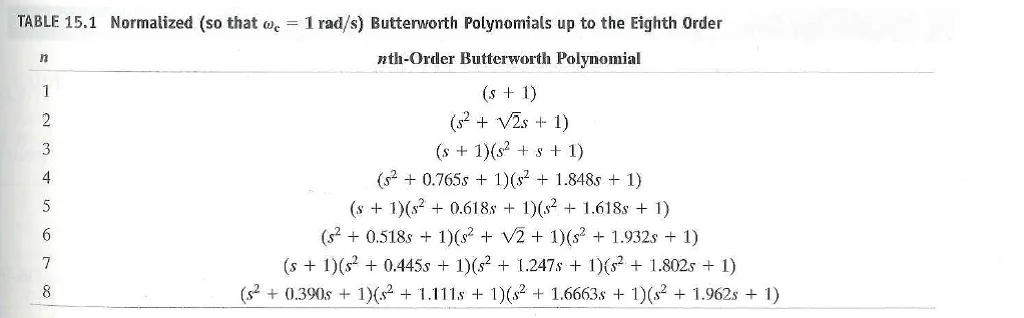
\includegraphics[width = 7in]{/home/zachariahmus/Documents/Code_Projects/ECE351/ECE351/LabFinal/4643-1-1EEI29.png}
\end{center}

We first design our components to match the polynomial values, then shift the values based on the frequency and magnitude scaling. 

\subsection*{Scaling}

In order to scale each of our component values, there are formulas for each component type: 
$$R'=Rk_m$$
$$C'=\frac{C}{k_mk_f}$$
$$L' = \frac{k_m}{k_f}L$$

\subsection*{Low-Pass Stage}
\begin{center}
	The general form of a butterworth low pass filter of our topology looks like: 
$$\frac{\frac{1}{R^2C_1C_2}}{s^2+\frac{2}{RC_1}s+\frac{1}{R^2C_1C_2}}$$
If we then add our scaling factors into the mix:
$$\frac{\frac{1}{(Rk_m)^2\frac{C_1C_2}{(k_mk_f)^2}}}{s^2+\frac{2}{Rk_m\frac{C_1}{k_mk_f}}s+\frac{1}{(Rk_m)^2\frac{C_1C_2}{(k_mk_f)^2}}}$$
If we simplify and use 1\Omega\ as our prototype value for our resistors we get:
$$\frac{\frac{k_f^2}{C_1C_2}}{s^2+\frac{2k_f}{C_1}s+\frac{k_f^2}{C_1C_2}}$$
\end{center}
\subsection*{High-Pass Stage}
\begin{center}
The general form of a butterworth high pass filter of our topology looks like:
$$\frac{s^2}{s^2+\frac{2}{R_1C}s+\frac{1}{R_1R_2C^2}}$$
If we then add our scaling factors into the mix:
$$\frac{s^2}{s^2+\frac{2}{R_1k_m\frac{C}{k_mk_f}}s+\frac{1}{R_1R_2k_m^2\frac{C^2}{k_m^2k_f^2}}}$$
If we simplify and use 1F as our prototype value for our capacitors we get:
$$\frac{s^2}{s^2+\frac{2k_f}{R_1}s+\frac{k_f^2}{R_1R_2}}$$

If we use 1F capacitors, we end up needing \mu\Omega\ resistors, so we need to scale them down to \mu F capacitors to allow our resistor values to grow by a factor of 1,000,000 and be in the range of purchasable resistors.
\end{center}
\subsection*{Circuit}
Using both the prototype polynomials and the component value functions, we can find values for each of the stages of the overall filter: 
\begin{center}
	{Figure 12.2}
	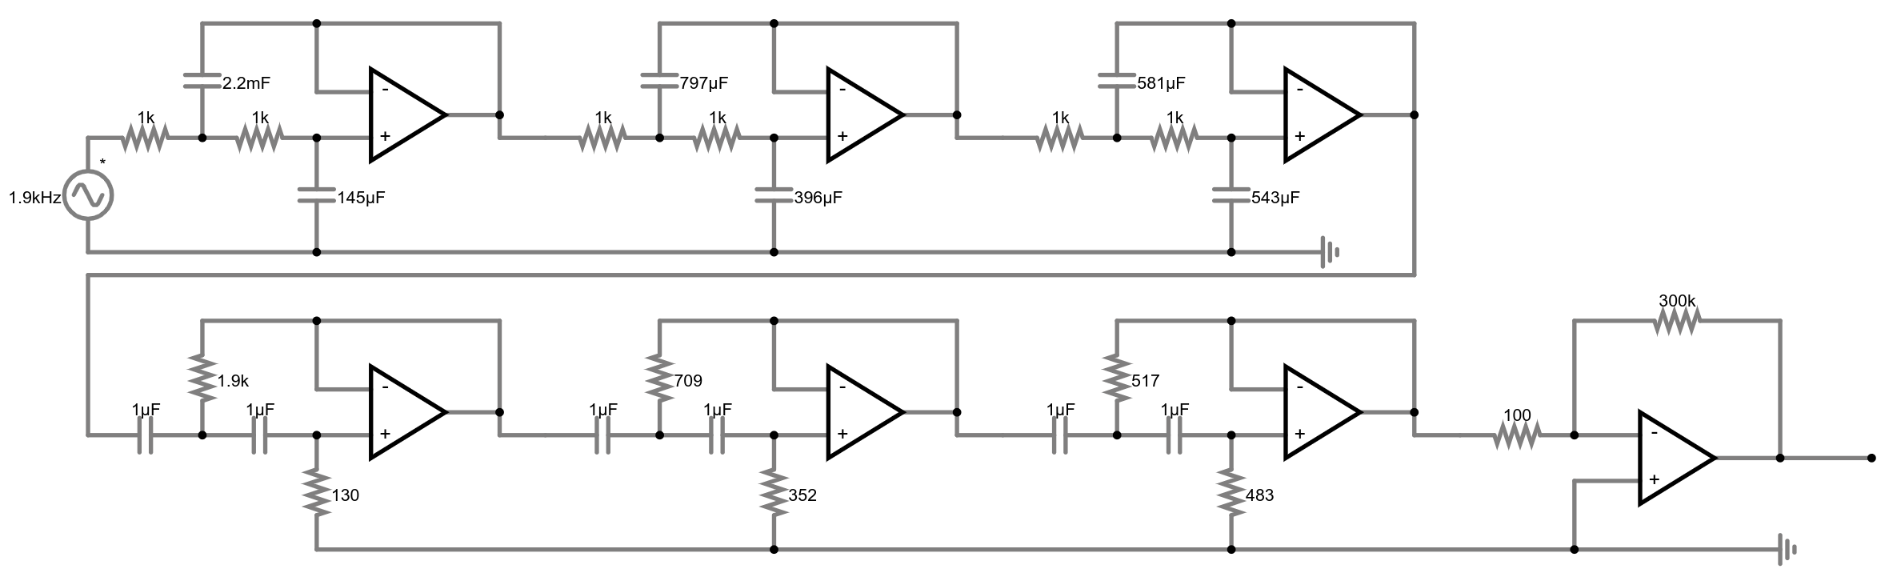
\includegraphics[width = 7in]{/home/zachariahmus/Documents/Code_Projects/ECE351/ECE351/LabFinal/2023-04-25_13-24.png}
\end{center}
\vspace{12pt}

\section*{Transfer Functions}
Now that the filter stages have been created, we need to know their characteristics. Each of the first three second order stages add up to a 6th order low pass filter and the second 3 add up to a 6th order high pass filter. The bandpass region ends up being attenuated too much through just these, so a gain stage was introduced at the end to buffer the signal.
\begin{center}
	{Figure 12.3}
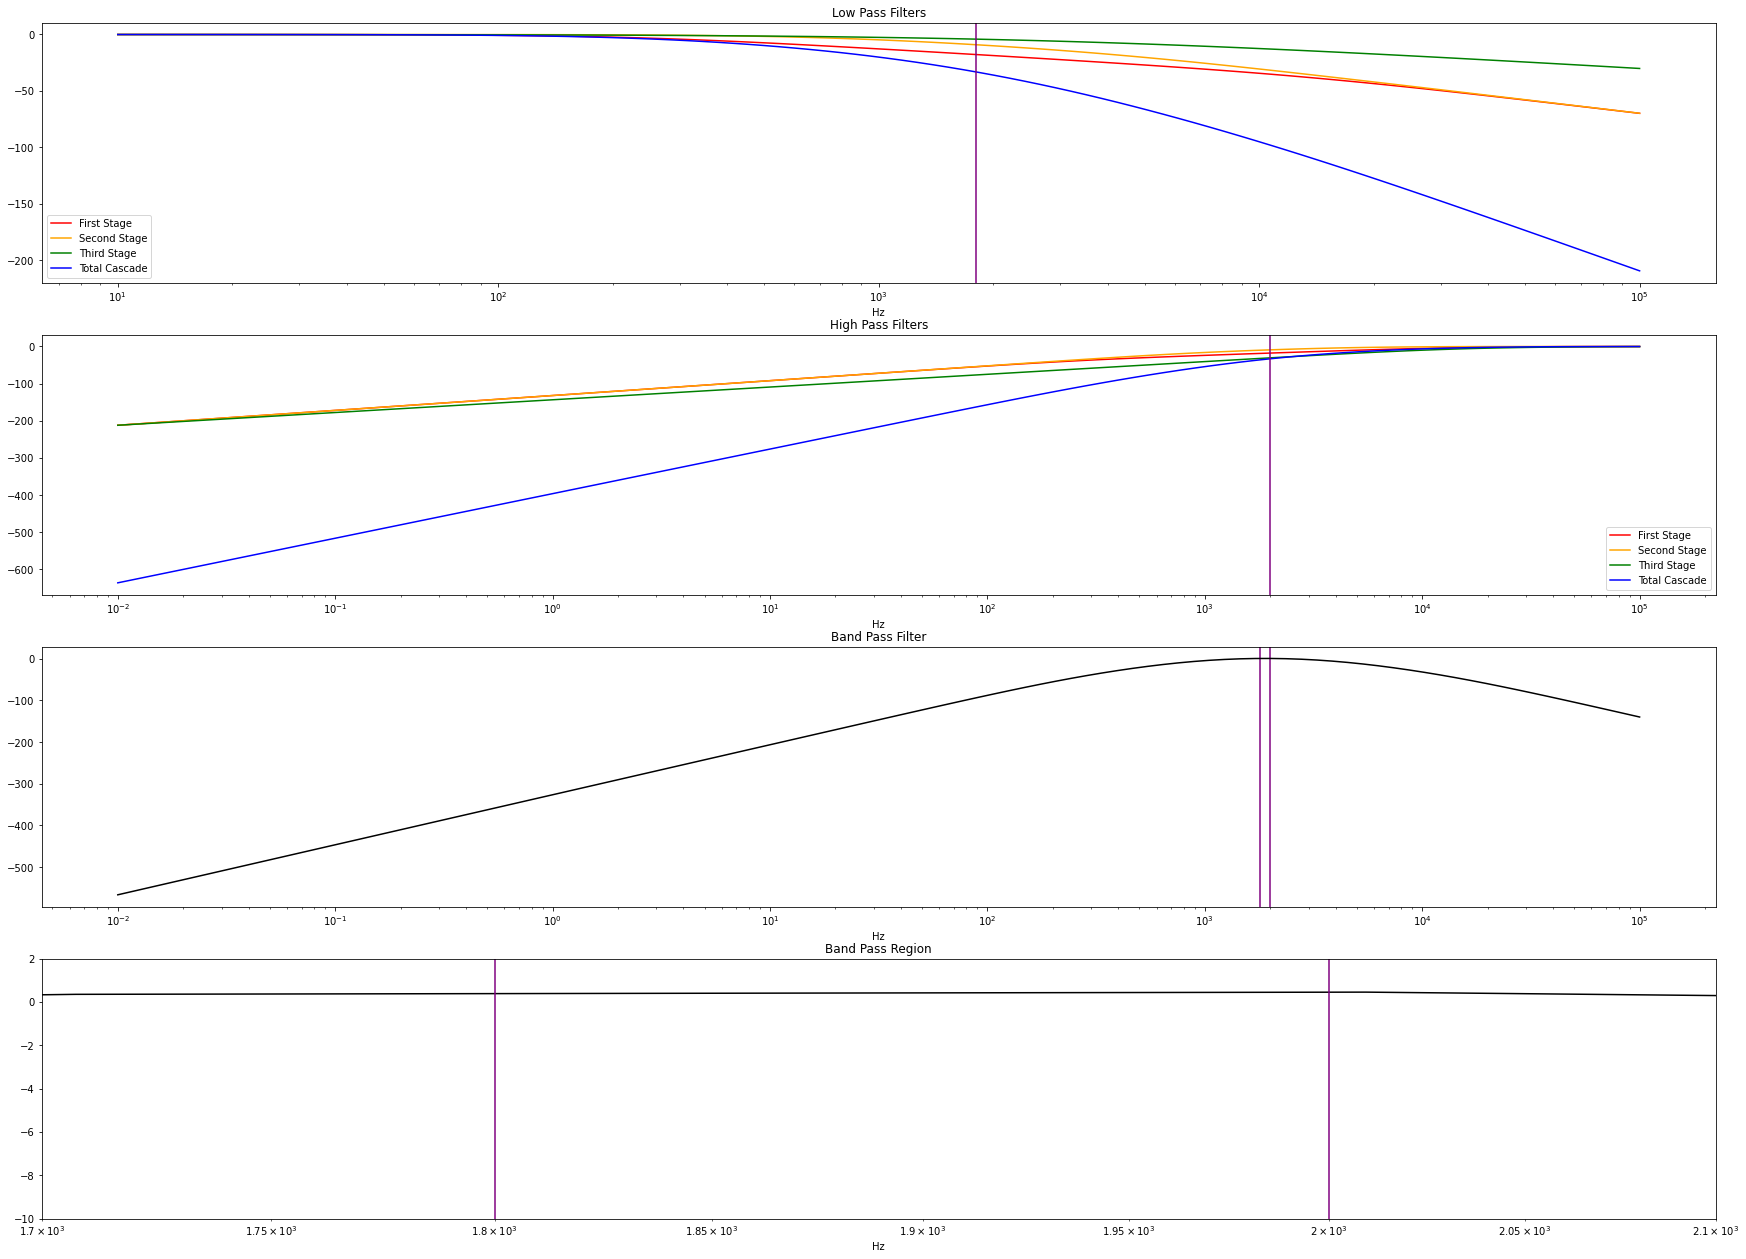
\includegraphics[width = 7in]{/home/zachariahmus/Documents/Code_Projects/ECE351/ECE351/LabFinal/Filter.png}
\end{center}
The low-pass stage has a cutoff frequency of 2000Hz and the highpass has a cutoff of 1800Hz, meaning anything in that region ends up slightly boosted whereas anything outside that region should be attenuated out. 
\section*{Testing and Verification}
To test the filter we can put in a random sample frequency into the filter and see what comes out the other end. To test the filter is working correctly, we need to see the dominant frequencies before and after going through the filter: 
\begin{center}
	{Figure 12.4}
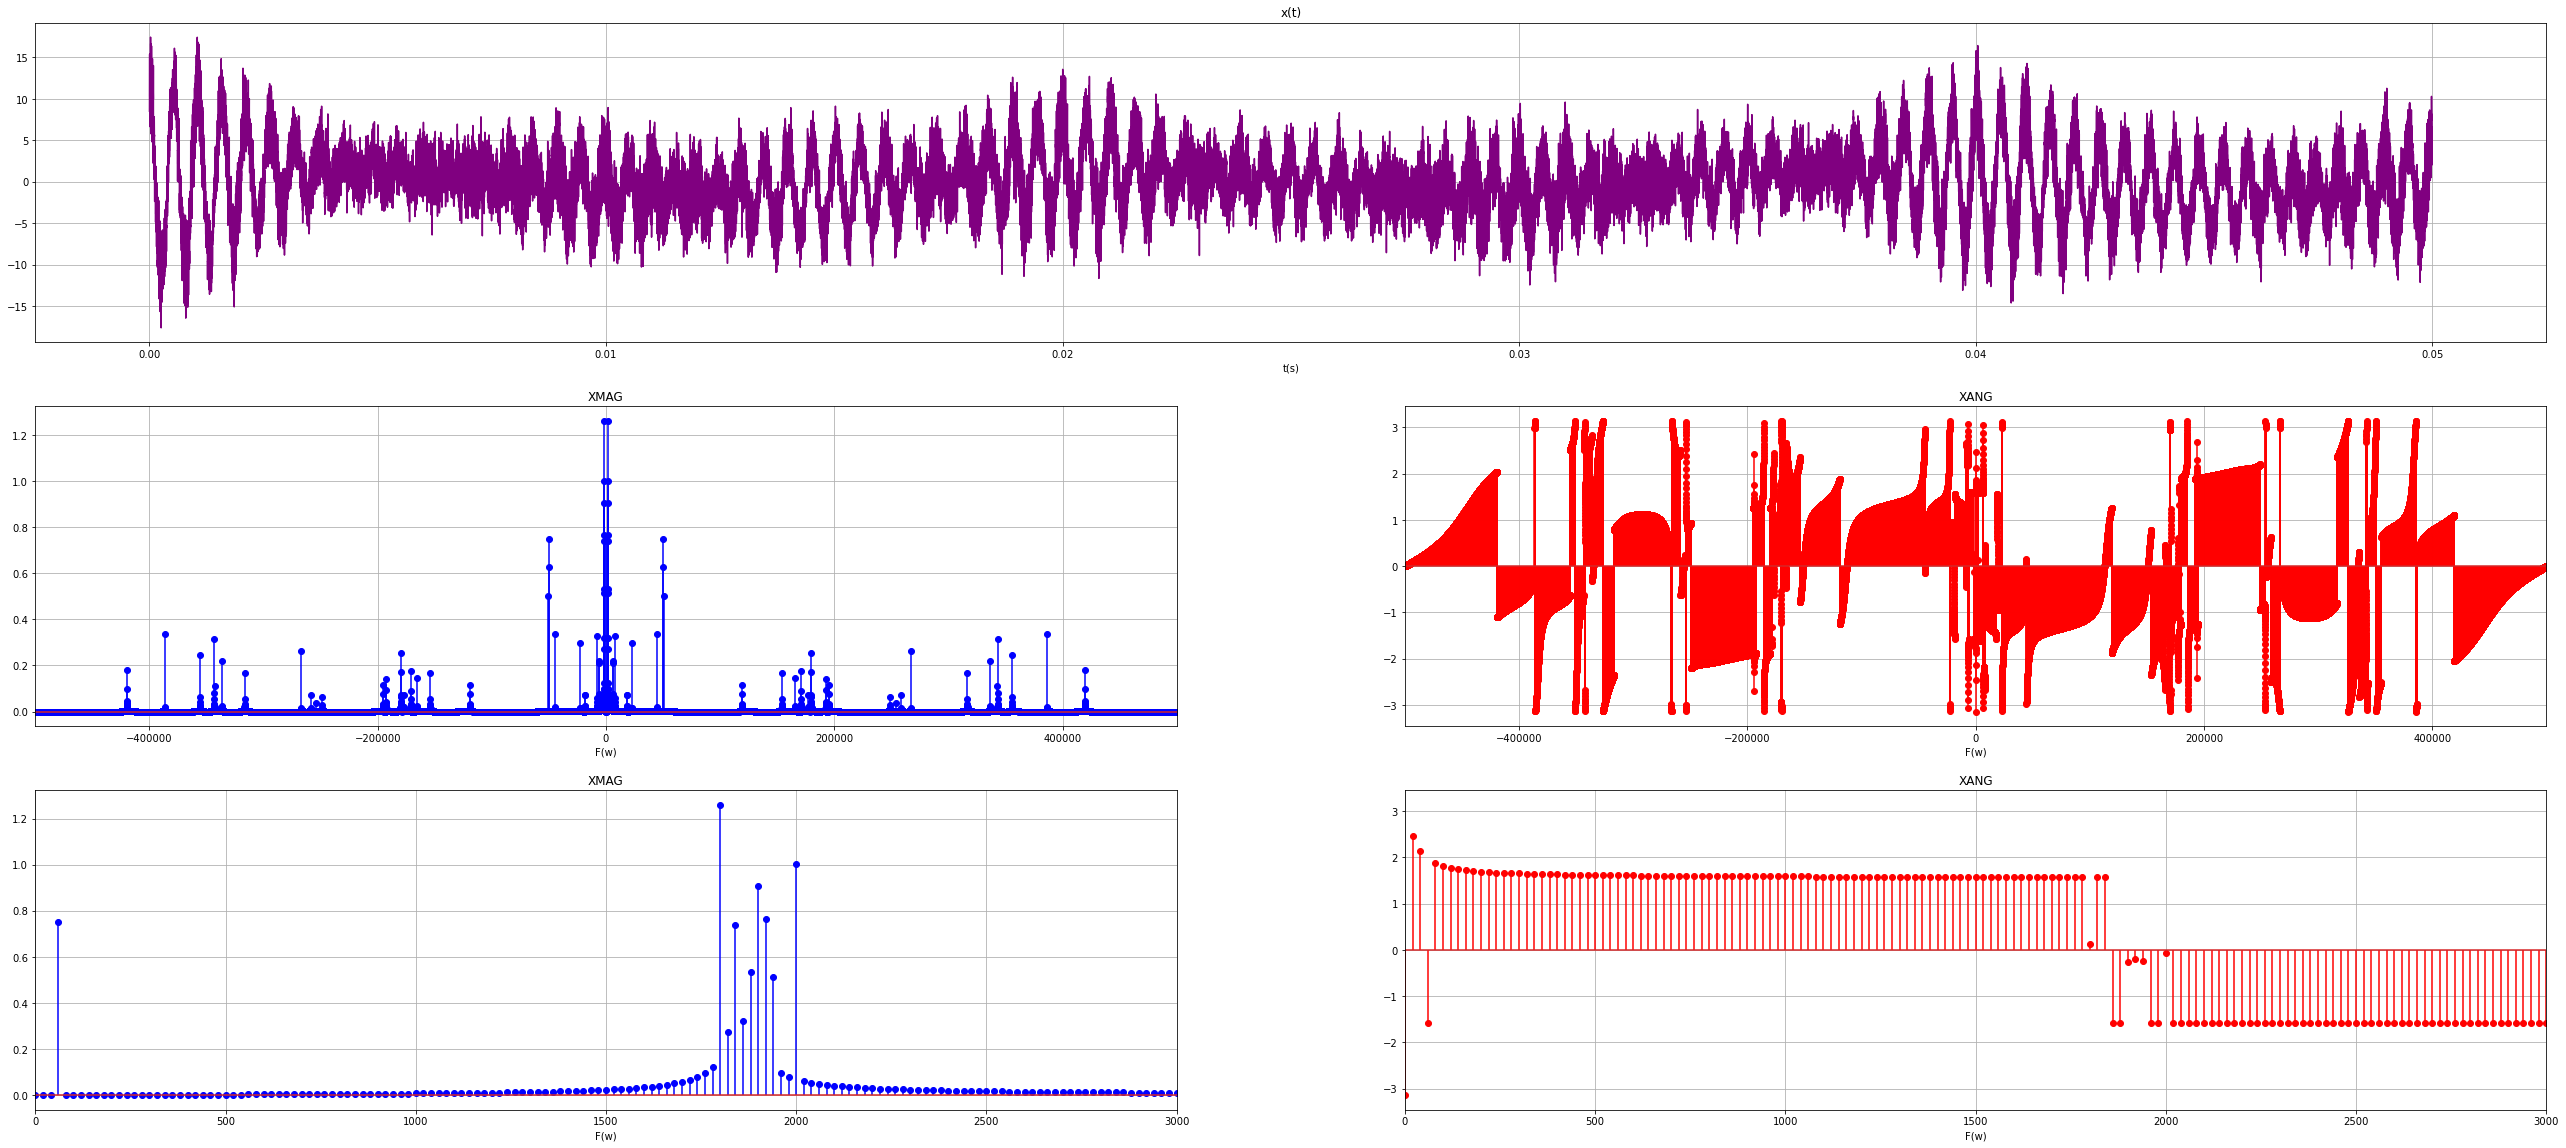
\includegraphics[width = 7in]{/home/zachariahmus/Documents/Code_Projects/ECE351/ECE351/LabFinal/Intro.png}
\end{center}
After going through the filter, the signal looks like: 
\begin{center}
	{Figure 12.5}
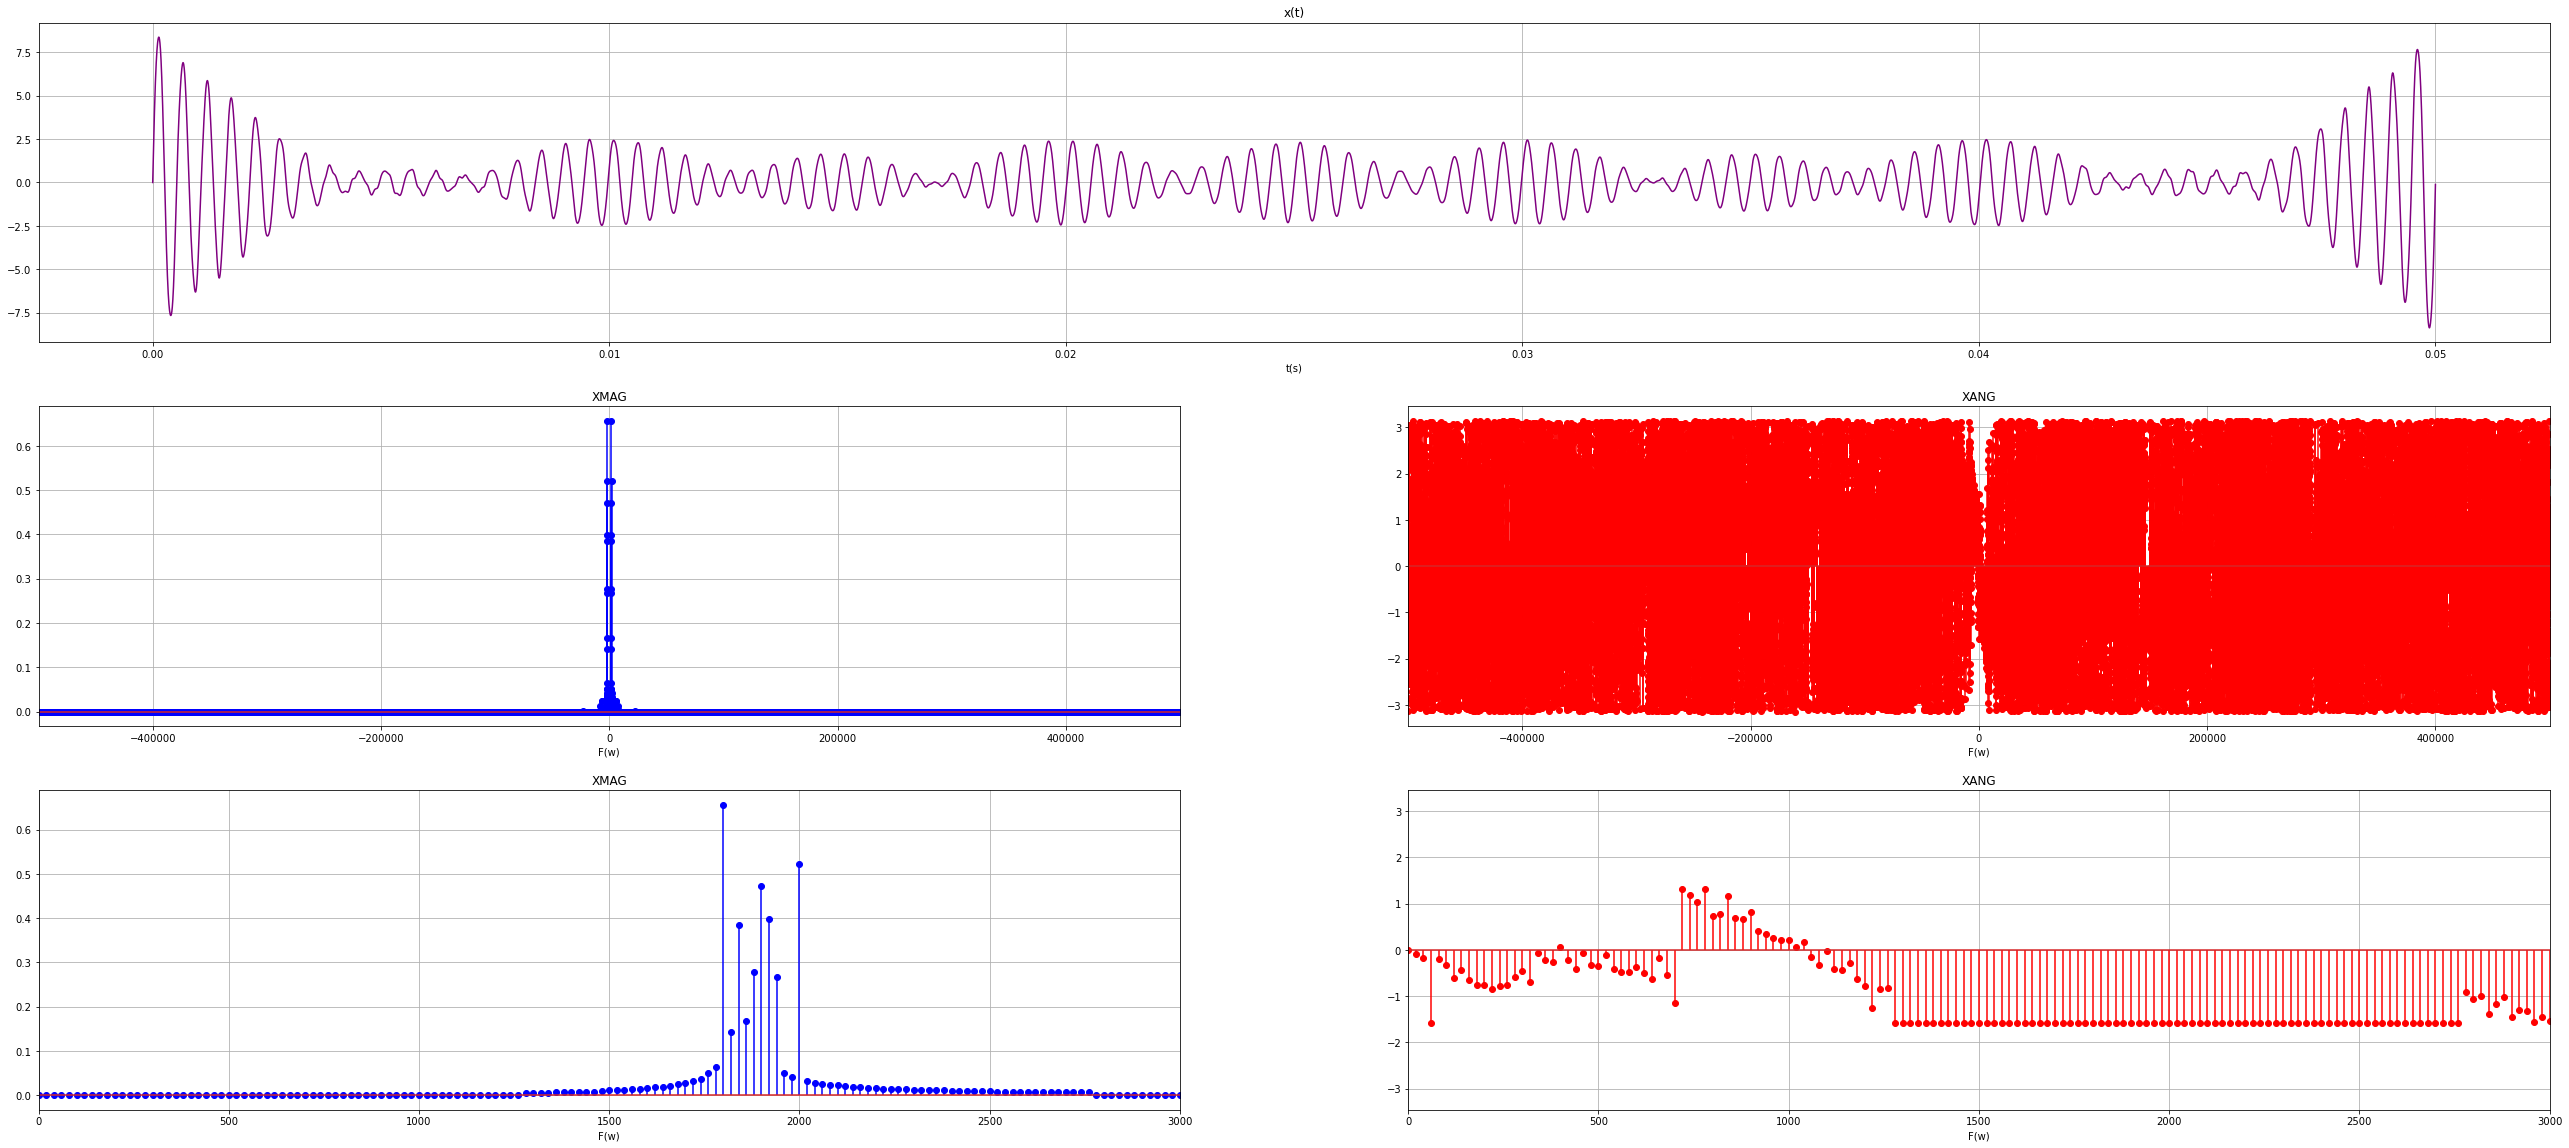
\includegraphics[width = 7in]{/home/zachariahmus/Documents/Code_Projects/ECE351/ECE351/LabFinal/Exit.png}

All of the frequencies other than those in the bandpass region are gone, and the signal looks much more normalized, showing that the filter has done exactly what it needs to do. 
\end{center}
\section*{Post Lab Questions}
Earlier this semester, you were asked what you personally wanted to get out of taking this
course. Do you feel like that personal goal was met? Why or why not?\vspace{12pt}

I wanted to come out of this course with experience in python, as signal processing may or may not be a tool I need but python is a versatile language that will give me a leg up in future classes or internships. To this end, I would say that my goal was met for this class. 
\section*{Conclusion}
In this lab we were able to create a filter for a system with specific demands. This lab was especially rewarding as we got to do some circuit design at then end, which seems more grounded and applicable than the other purely mathematical simulations we did in earlier labs. We worked with some circuits in other labs, but this is the first one we got to design. After being able to design the filter, we then had the tools to simulate and test it giving confirmation of both understanding and implementation. 
	
\end{document}
